\documentclass[a4paper, 11pt]{article}
\usepackage[utf8]{inputenc} % Change according your file encoding
\usepackage{graphicx}
\usepackage{url}

%opening
\title{Seminar Report: Paxy}
\author{Maria Gabriela Valdes and Victoria Beleuta}
\date{\today{}}

\begin{document}

\maketitle

\section{Introduction}

This assignment gave us the opportunity to learn and implement the \textit{Paxos} algorithm. This algorithm is a protocol for solving consensus between processes in a distributed system. Consensus consists in agreeing on a proposed value among a group of participants. In this particular case, we have a set of \textit{Proposers} that propose different values, to a set of \textit{Acceptors} until a single and unique value is agreed between all \textit{Proposers} and \textit{Acceptors}.

\section{Work done}

We have completed the code files provided to correctly implement the algorithm. Our source code consists of two folders: \textit{src} and \textit{src-sep}. The first one contains the erlang files implementig the Paxos algorithm with both proposers and acceptors starting in the same instance. The folder \textit{src-sep} we have modules to give the possibility to start the proposers in one machine and the acceptors in a different machine.

\section{Experiments}

First we run an experiment in the same machine with 3 proposers and 5 acceptors. After compiling the code files located in \textit{src} and running the paxy module \textit{paxy:start([200,200,200])}. Proposer 0, \textit{willard} proposes color \textit{blue}, and in round 2, the acceptors voted for \textit{kilgore} and decided on color \textit{blue}.\\
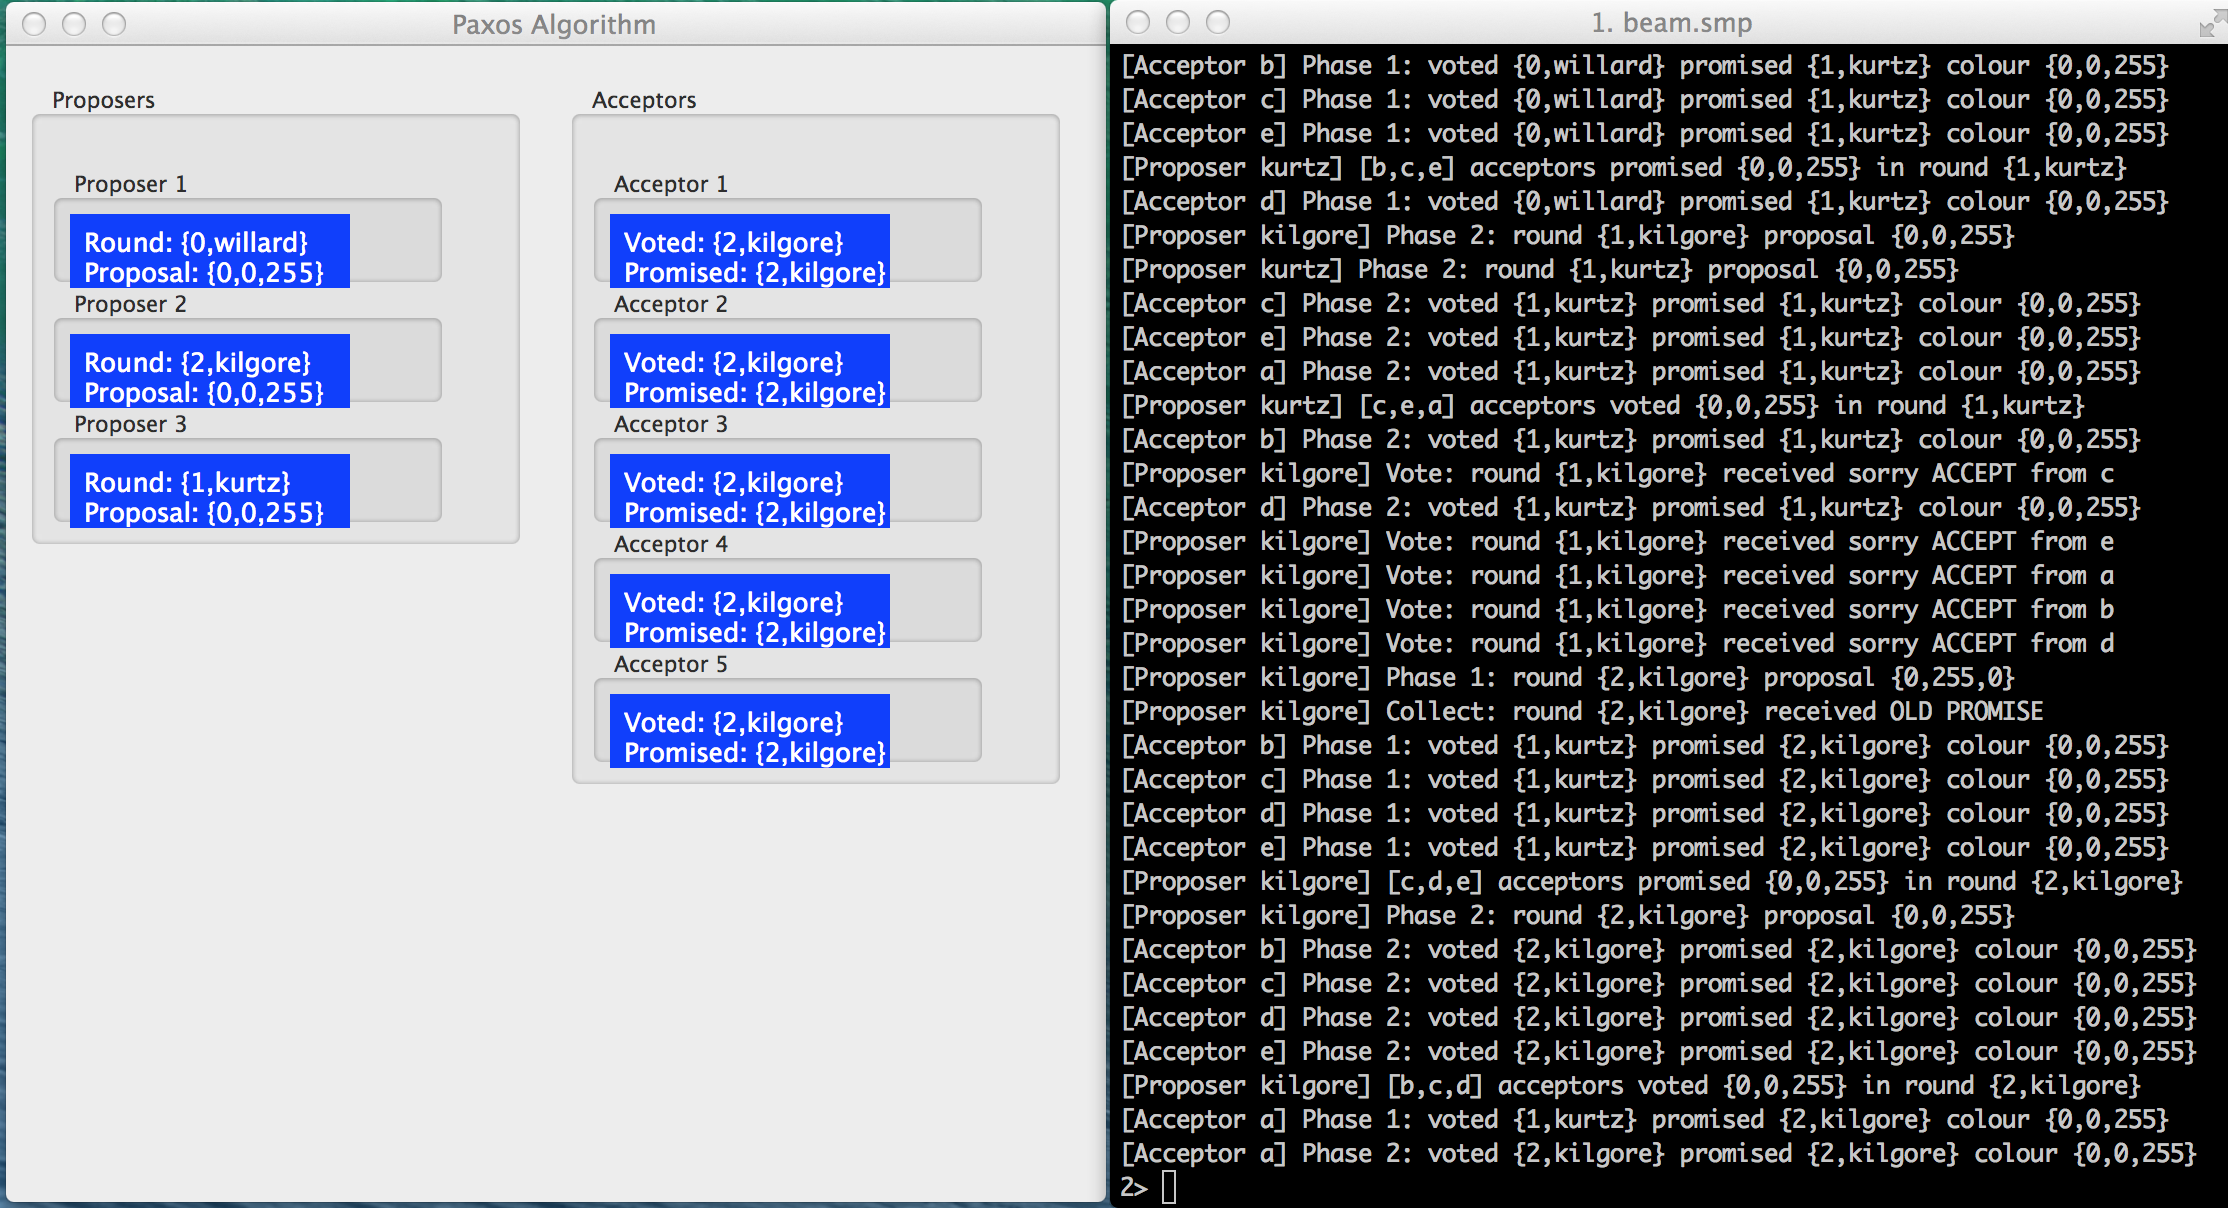
\includegraphics[scale=0.35]{images/exp0.png} \\\\

\textbf{i)} In this experiment we delay \textit{prepare} messages and we see that the algorithm terminates even with the delays shown in the trace.\\
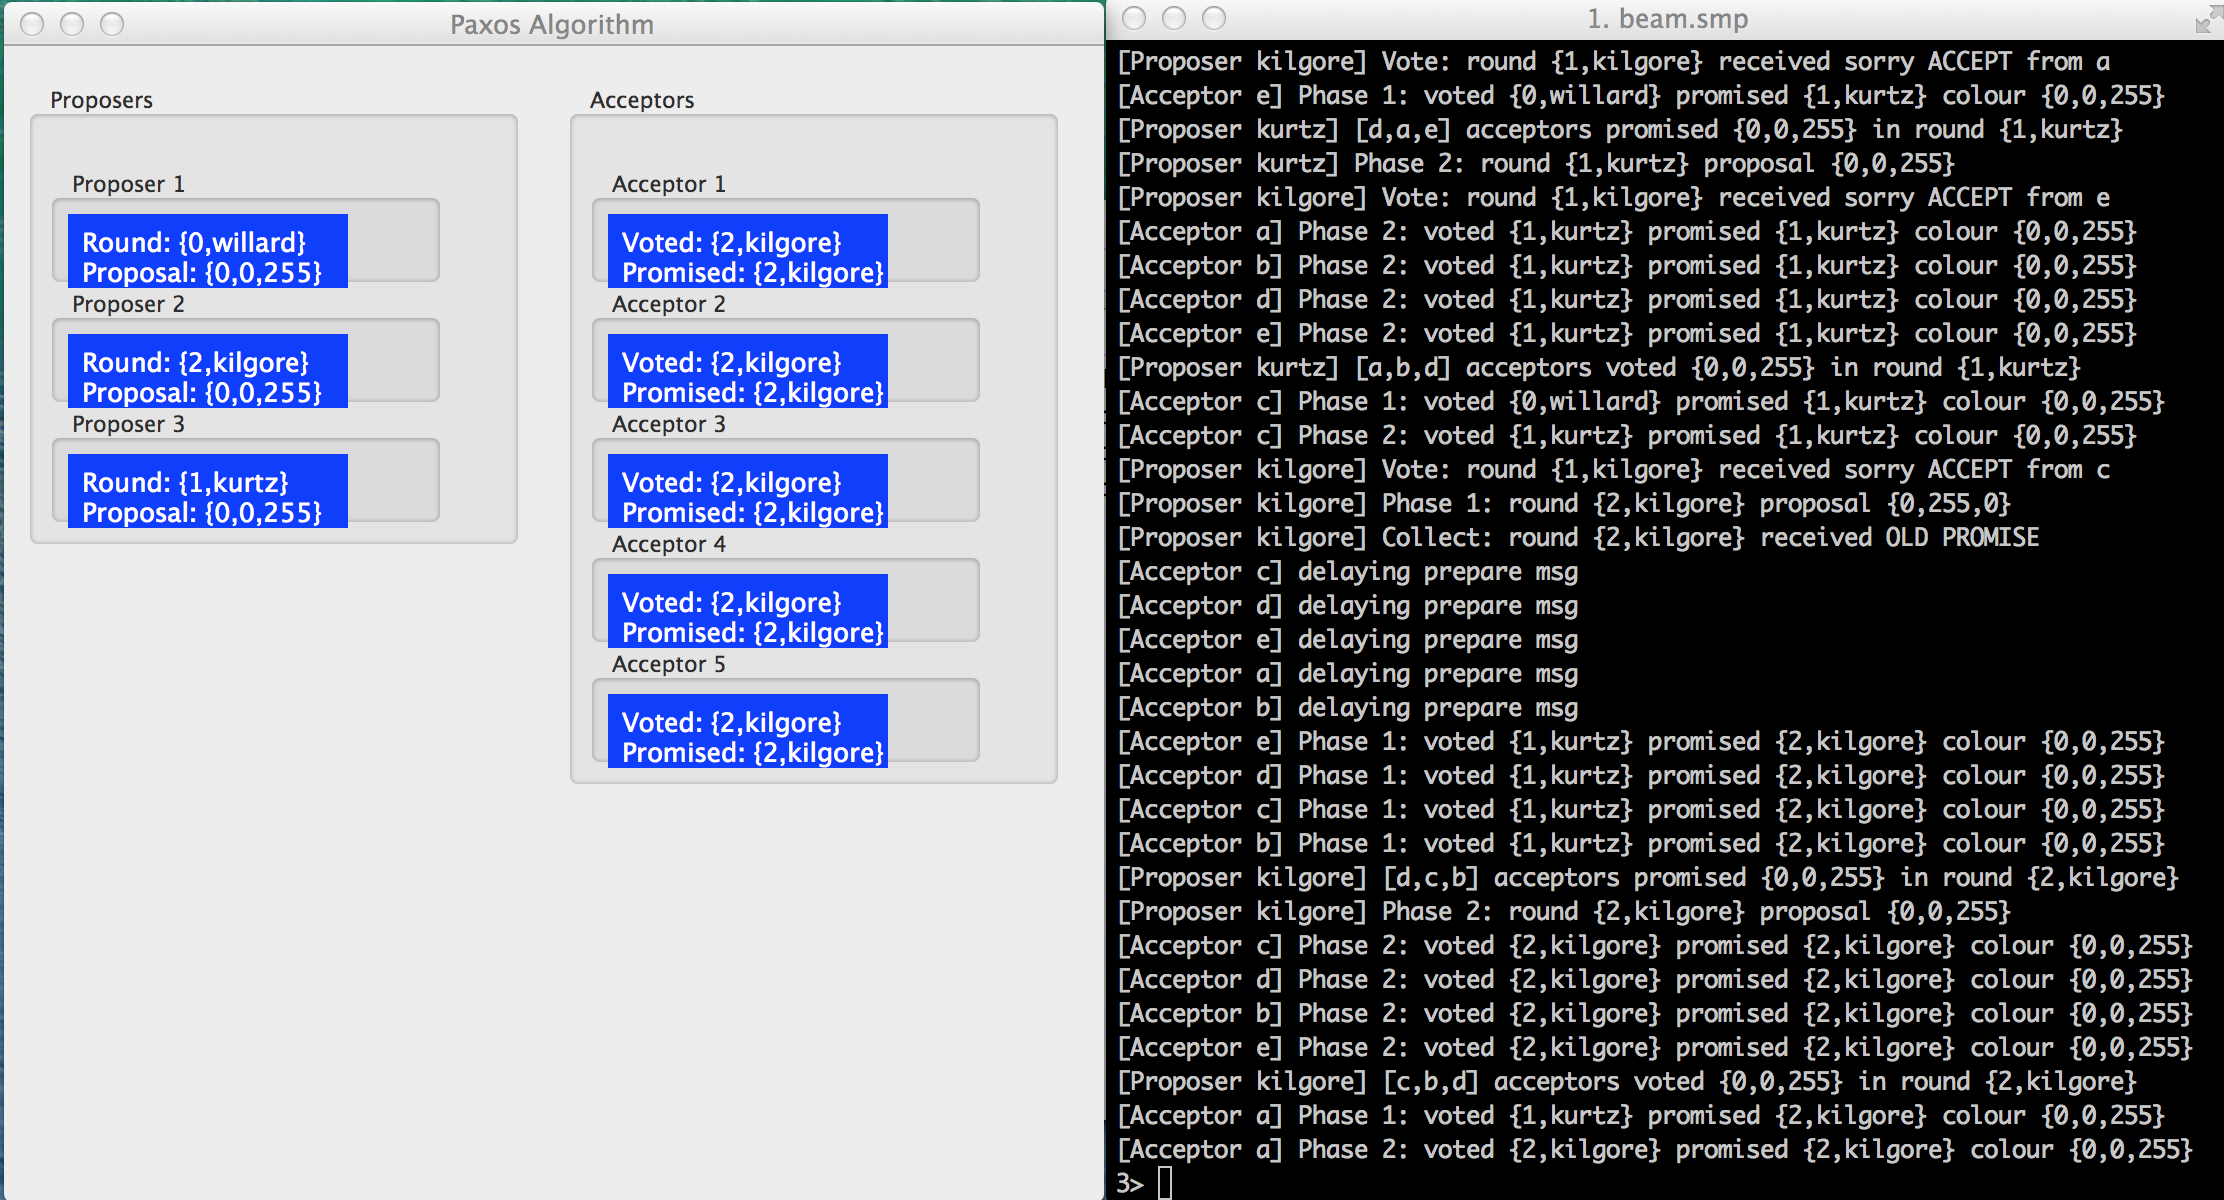
\includegraphics[scale=0.35]{images/exp1.png} \\\\
Now we add delays before the \textit{accept} messages, the algorithm terminates voting in round 2 for \textit{kilgore} and color \textit{blue}.\\
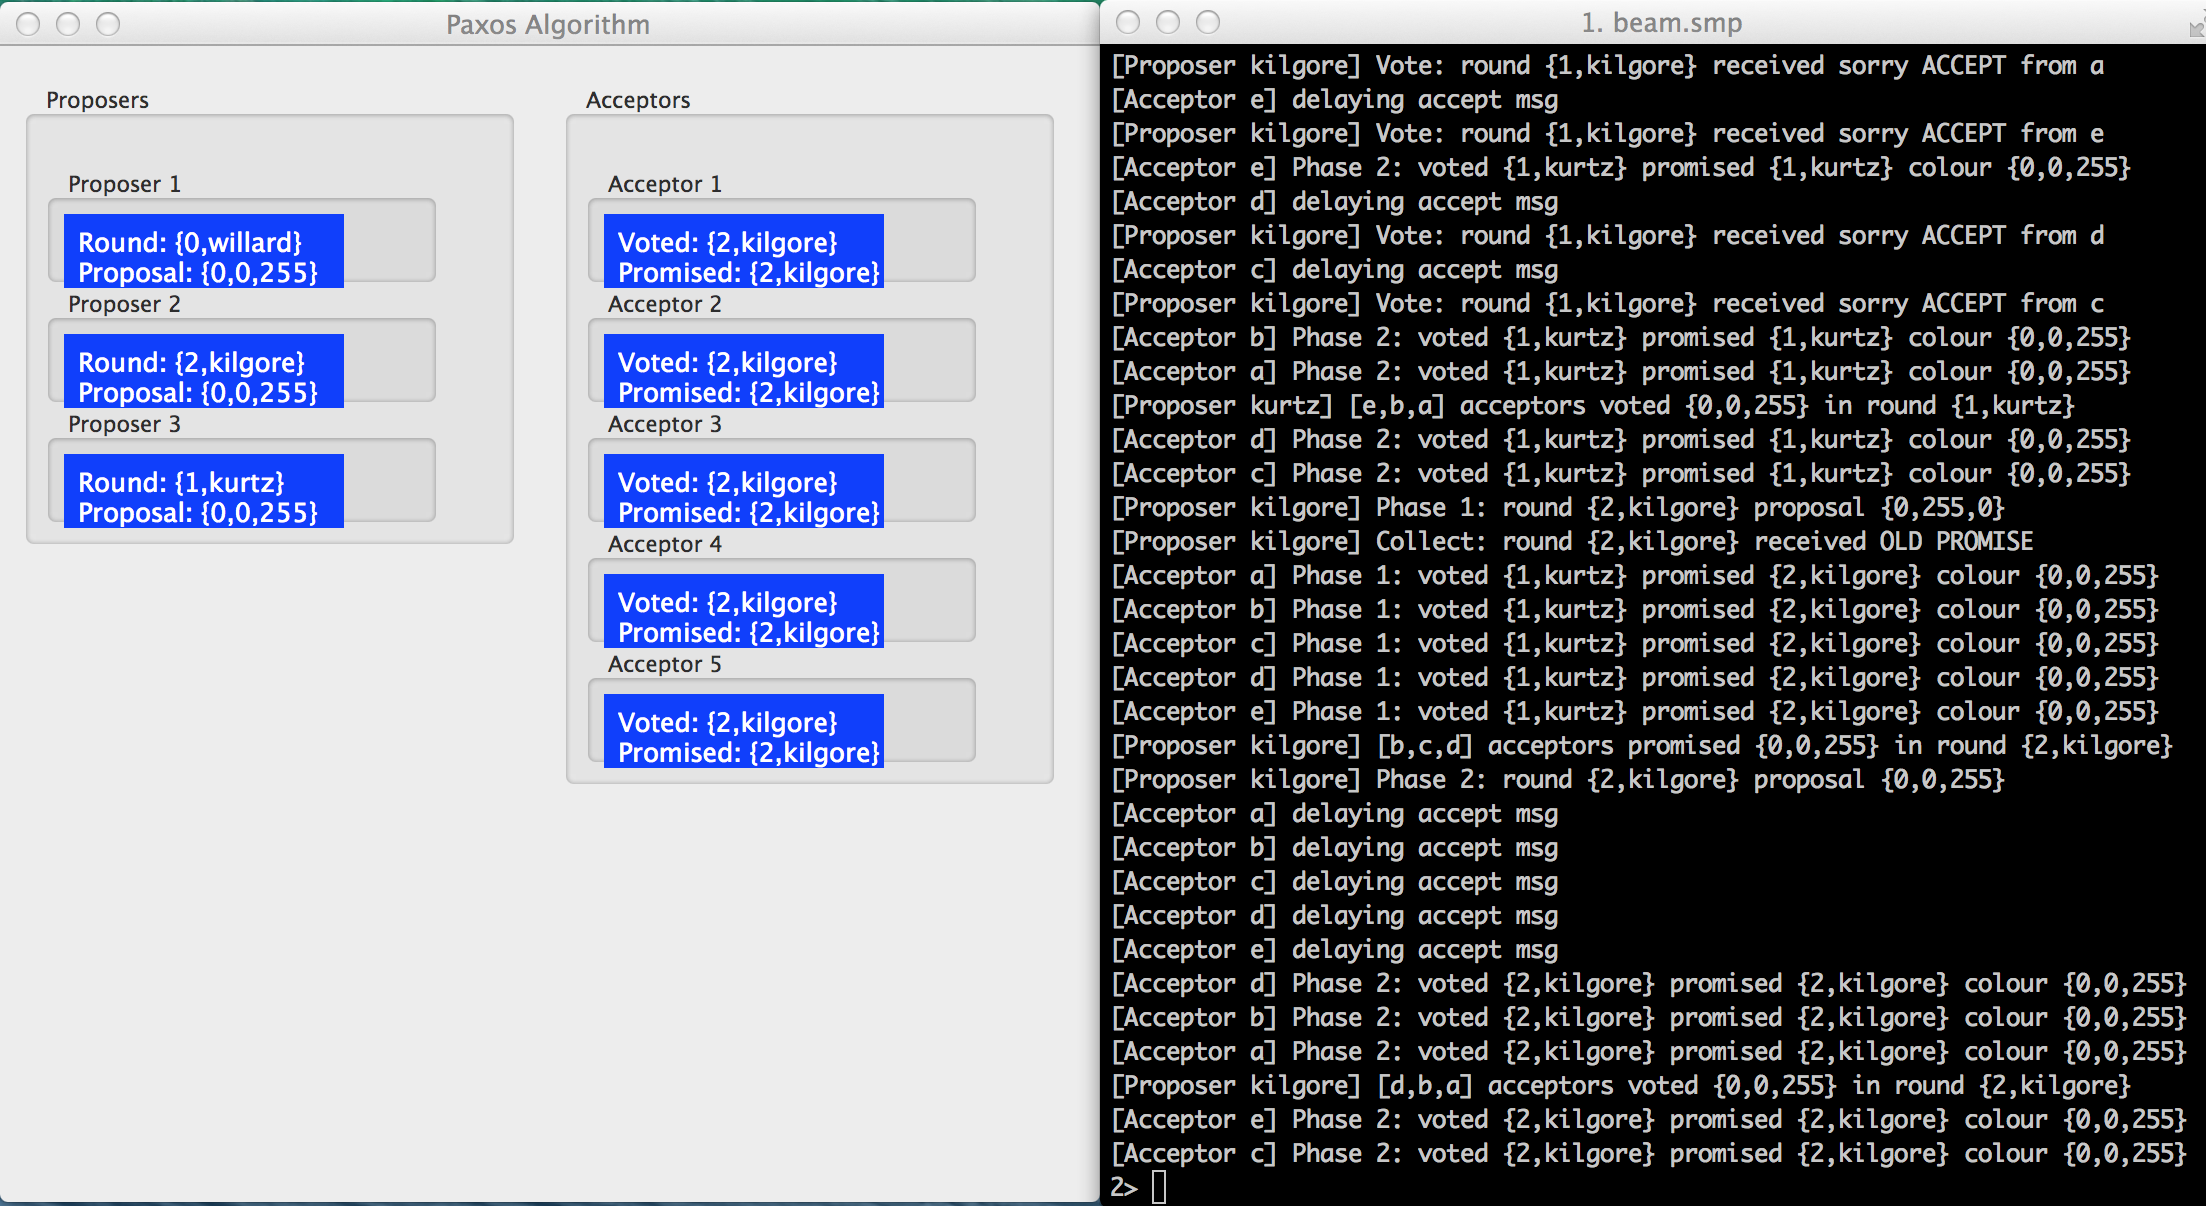
\includegraphics[scale=0.35]{images/exp2.png} \\\\
Lastly, we add delays both before \textit{prepare} and \textit{accept} messages and the acceptors reach the same consensus again.\\
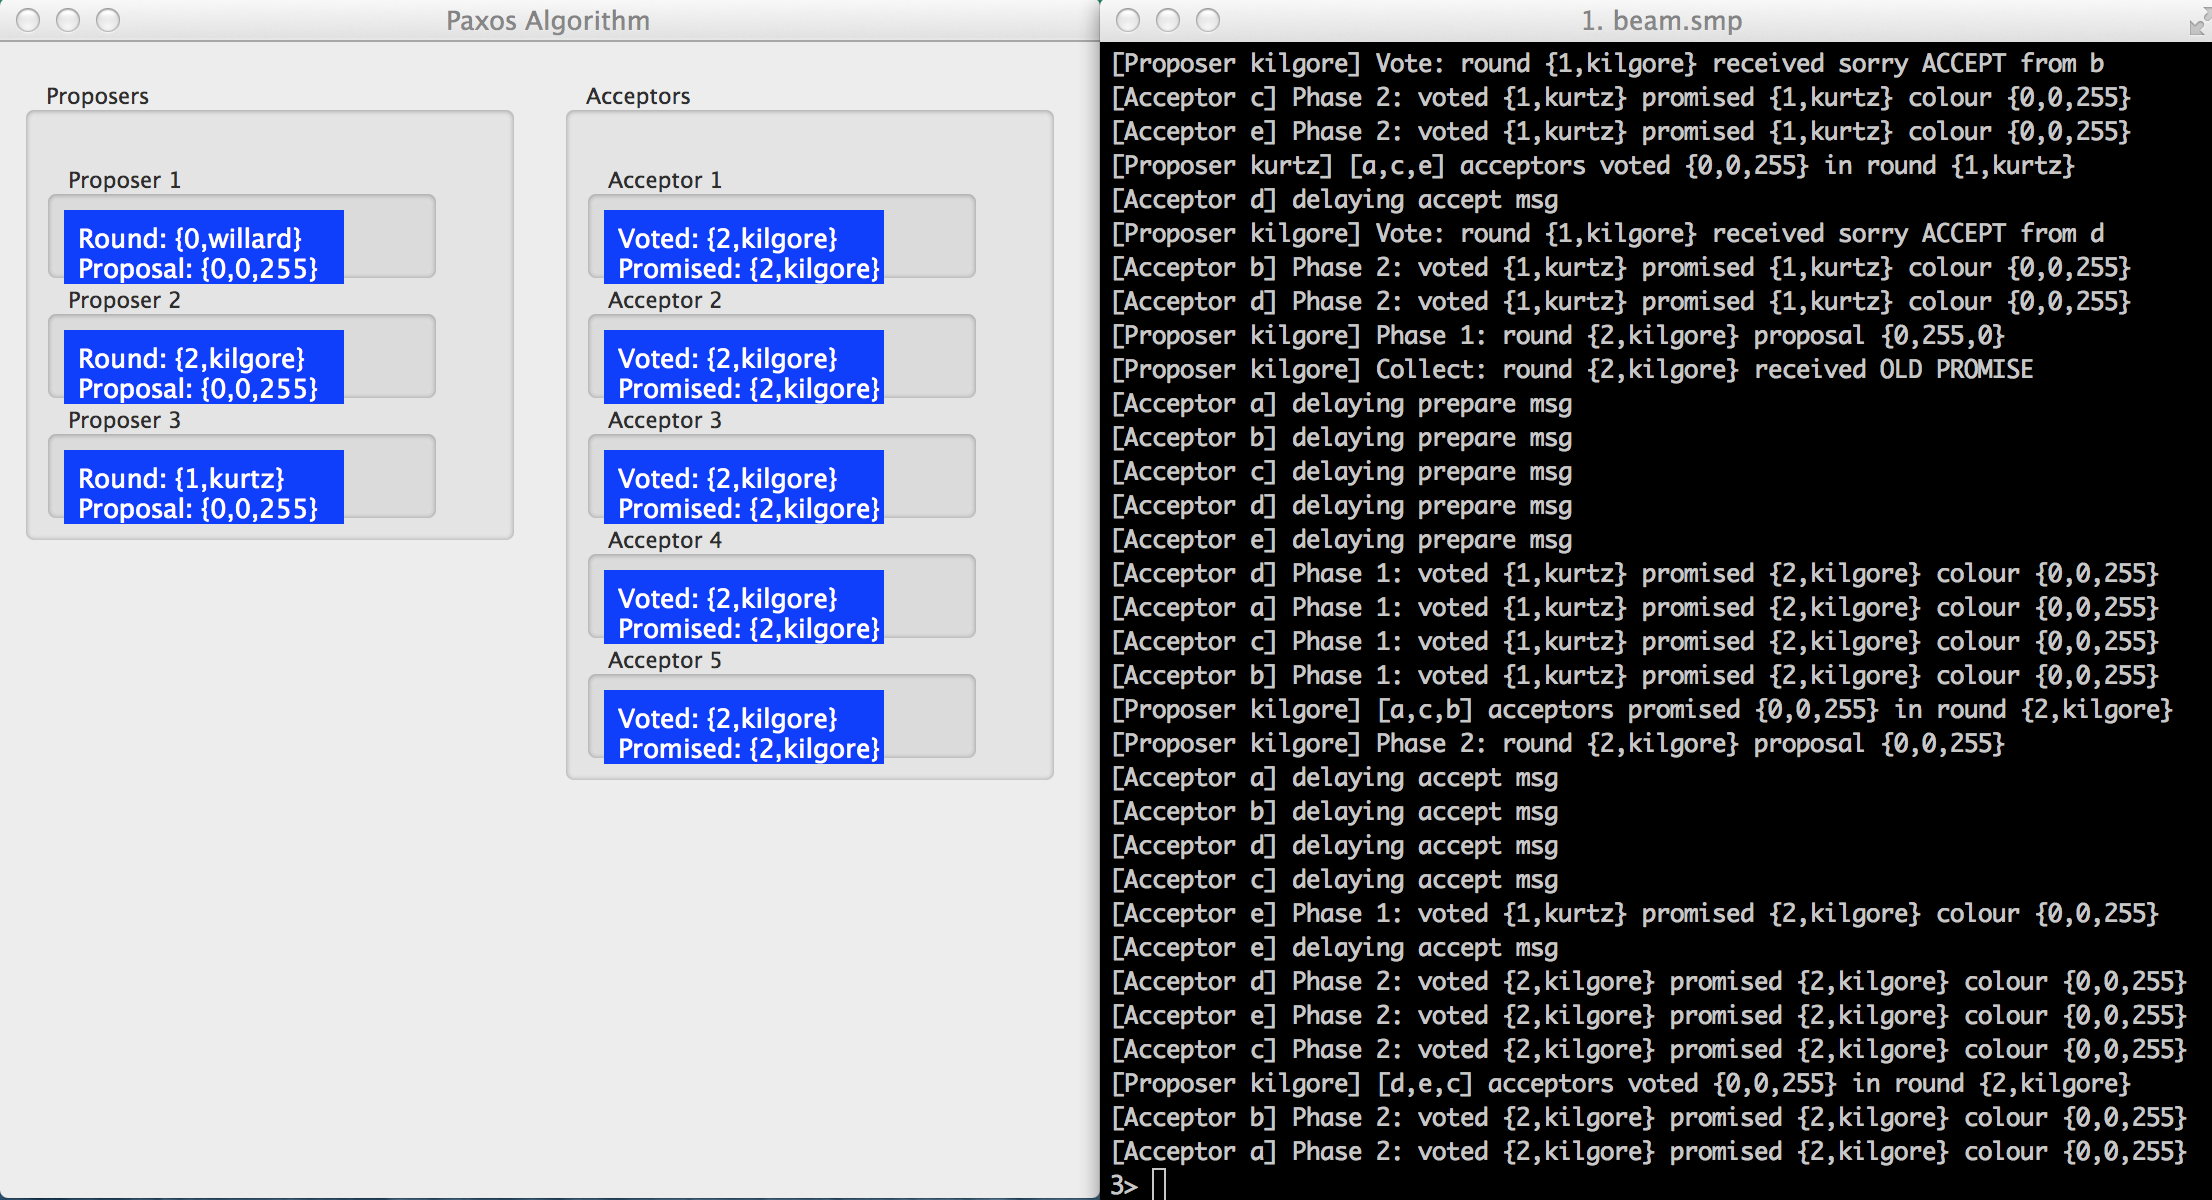
\includegraphics[scale=0.35]{images/exp3.png} \\\\

\textbf{ii)} We stop sending \textit{sorry} messages to the processor and we run the experiment to try to reach a consensus.\\
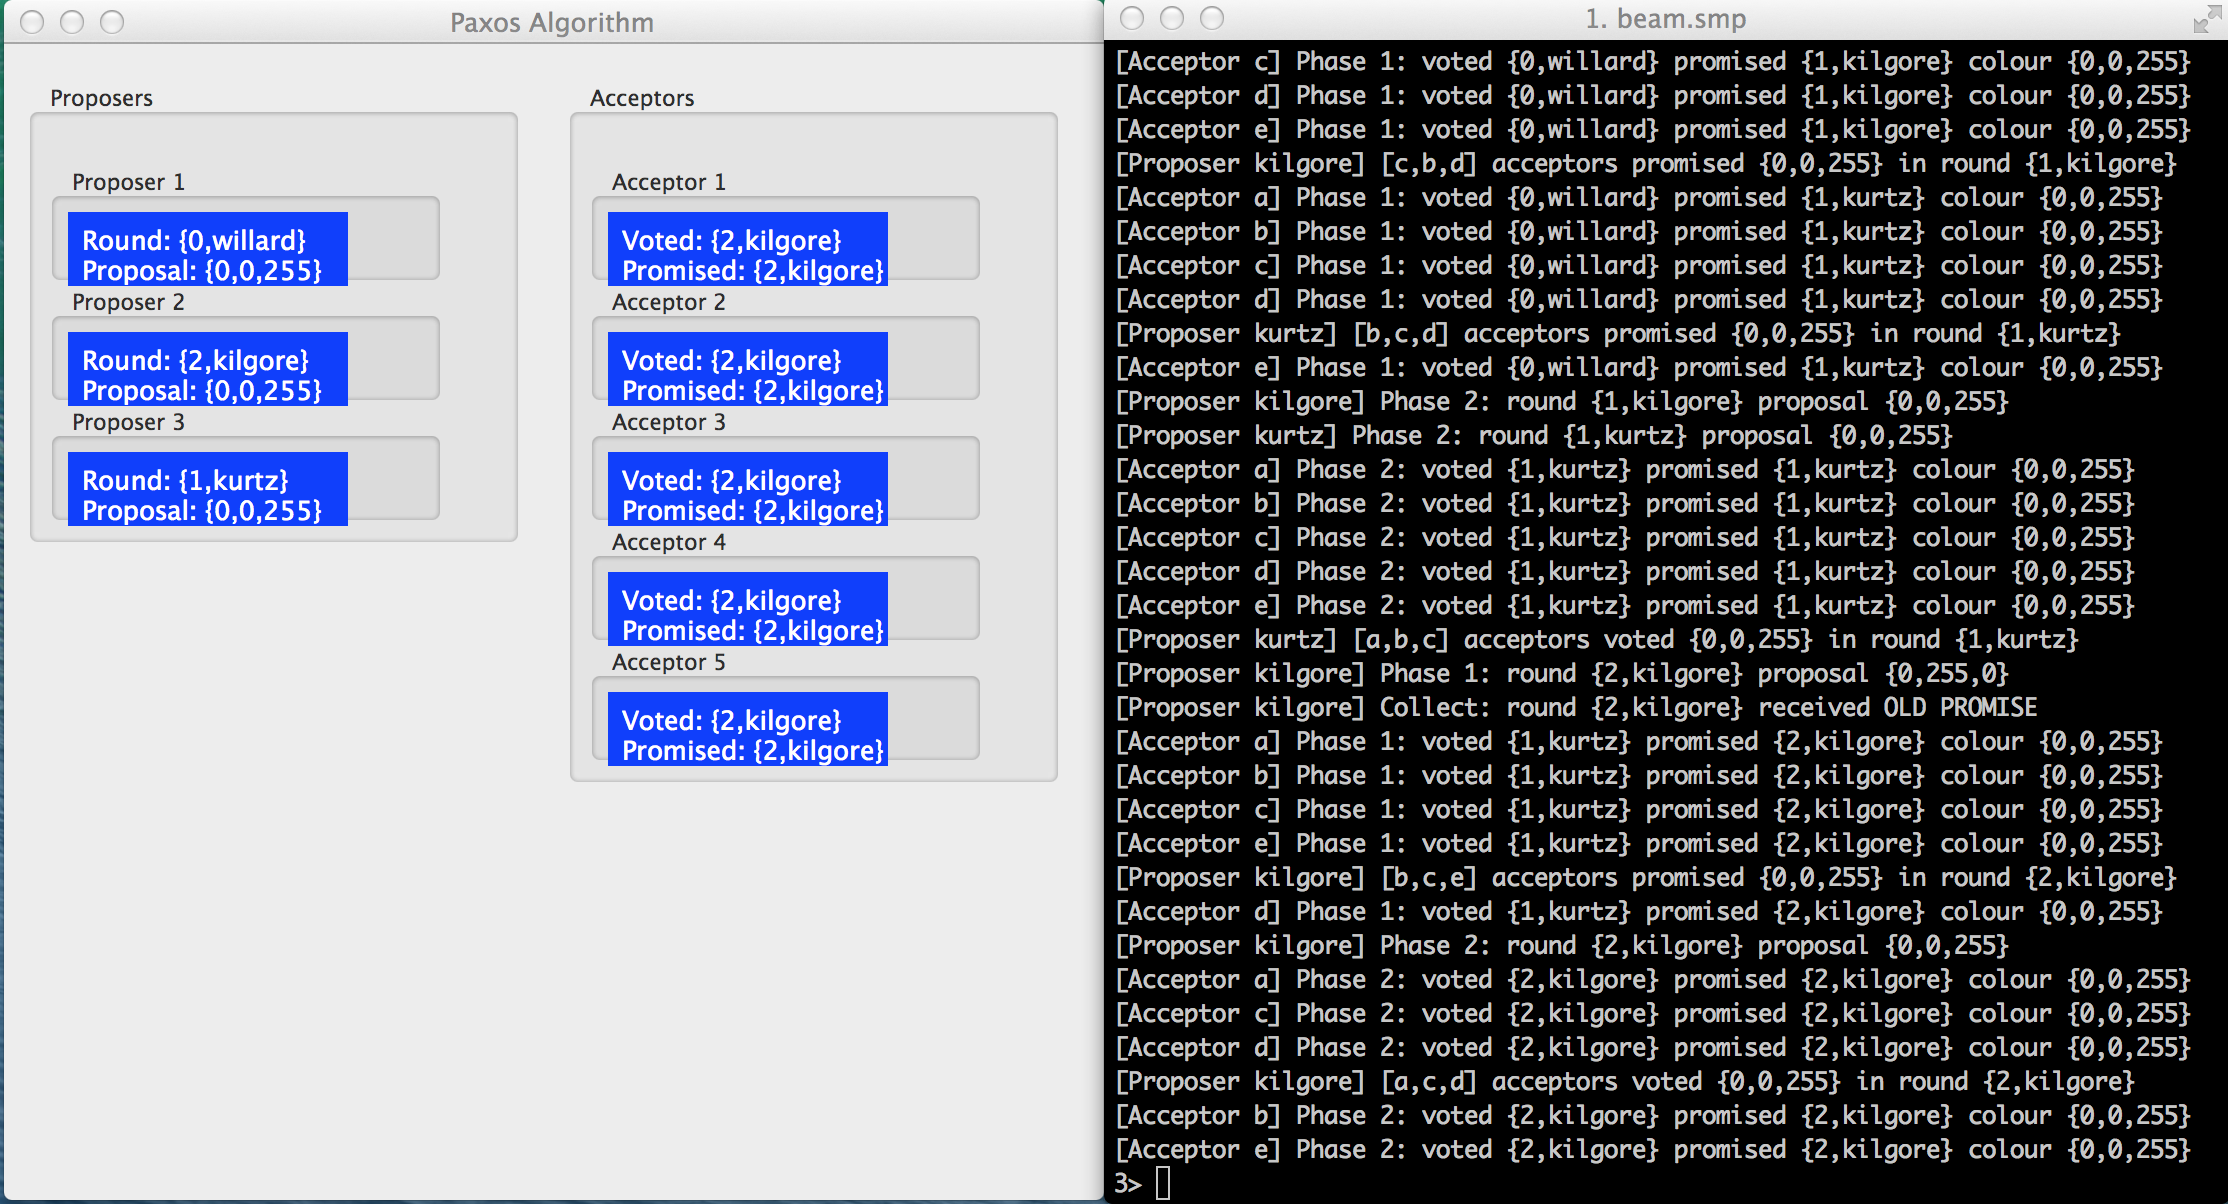
\includegraphics[scale=0.35]{images/exp4.png} \\\\

\textbf{iii)} In this experiment, we randomly drop \textit{promise} messages, and we look out for the consensus that the acceptors arrive to. Even though a promise message in round 2 is dropped, they still agree on the color blue.\\
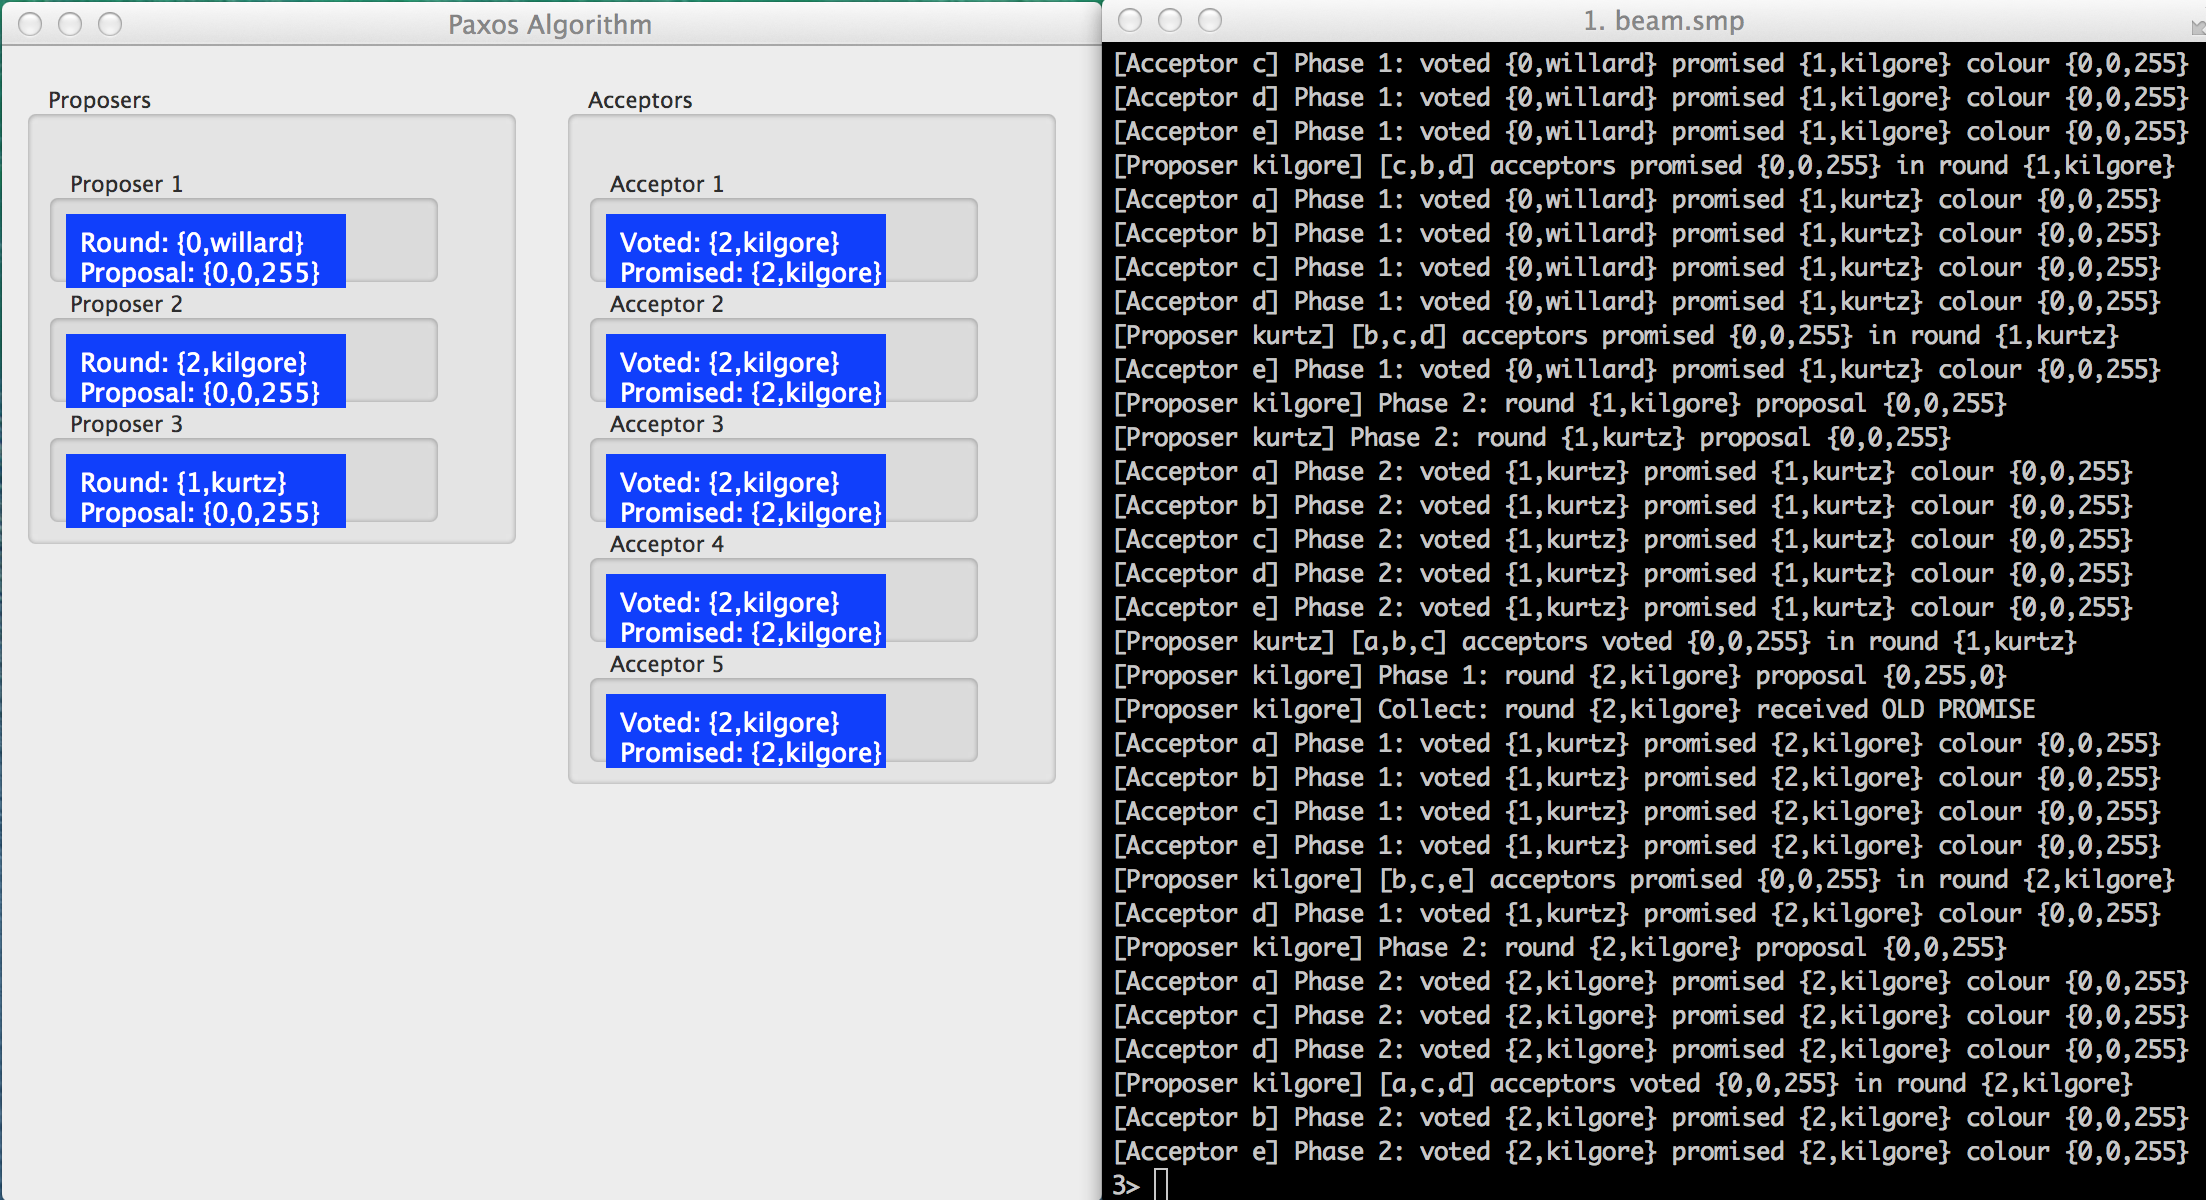
\includegraphics[scale=0.35]{images/exp5.png} \\\\
Now, we run an experiment droping \textit{vote} messages. Again, the acceptors manage to agree on the proposed color blue, even with a \textit{vote} message dropped because the other messages still amount to the majority of acceptors.\\
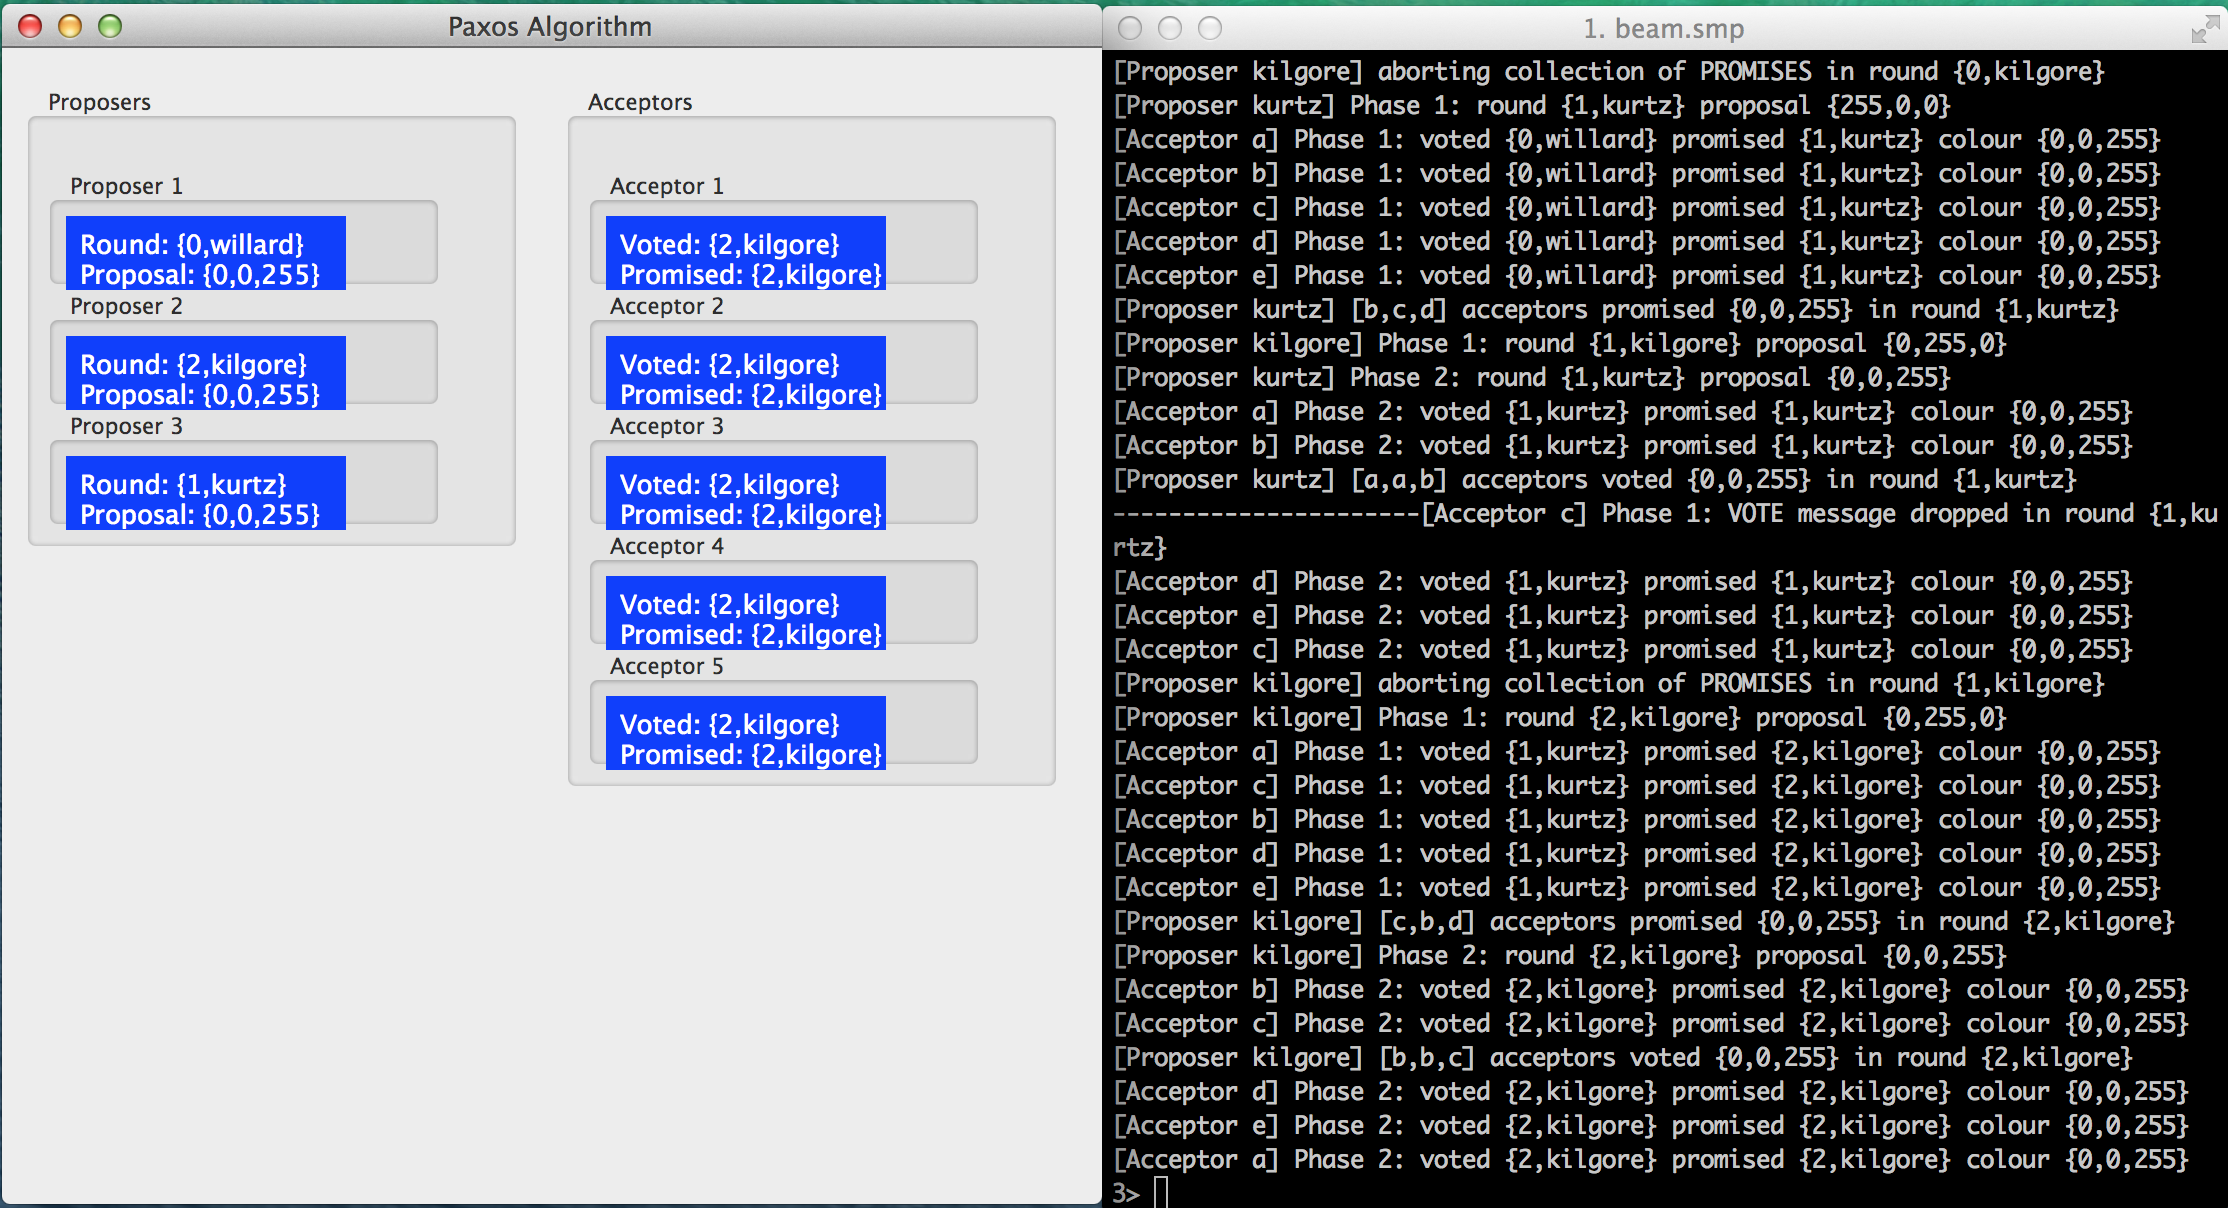
\includegraphics[scale=0.35]{images/exp6.png} \\\\
When we run the experiment dropping both \textit{promise} and \textit{vote} messages, we see that the algorithm still terminates successfully due to the fact that the majority of acceptors whose messages were not dropped agreed.\\
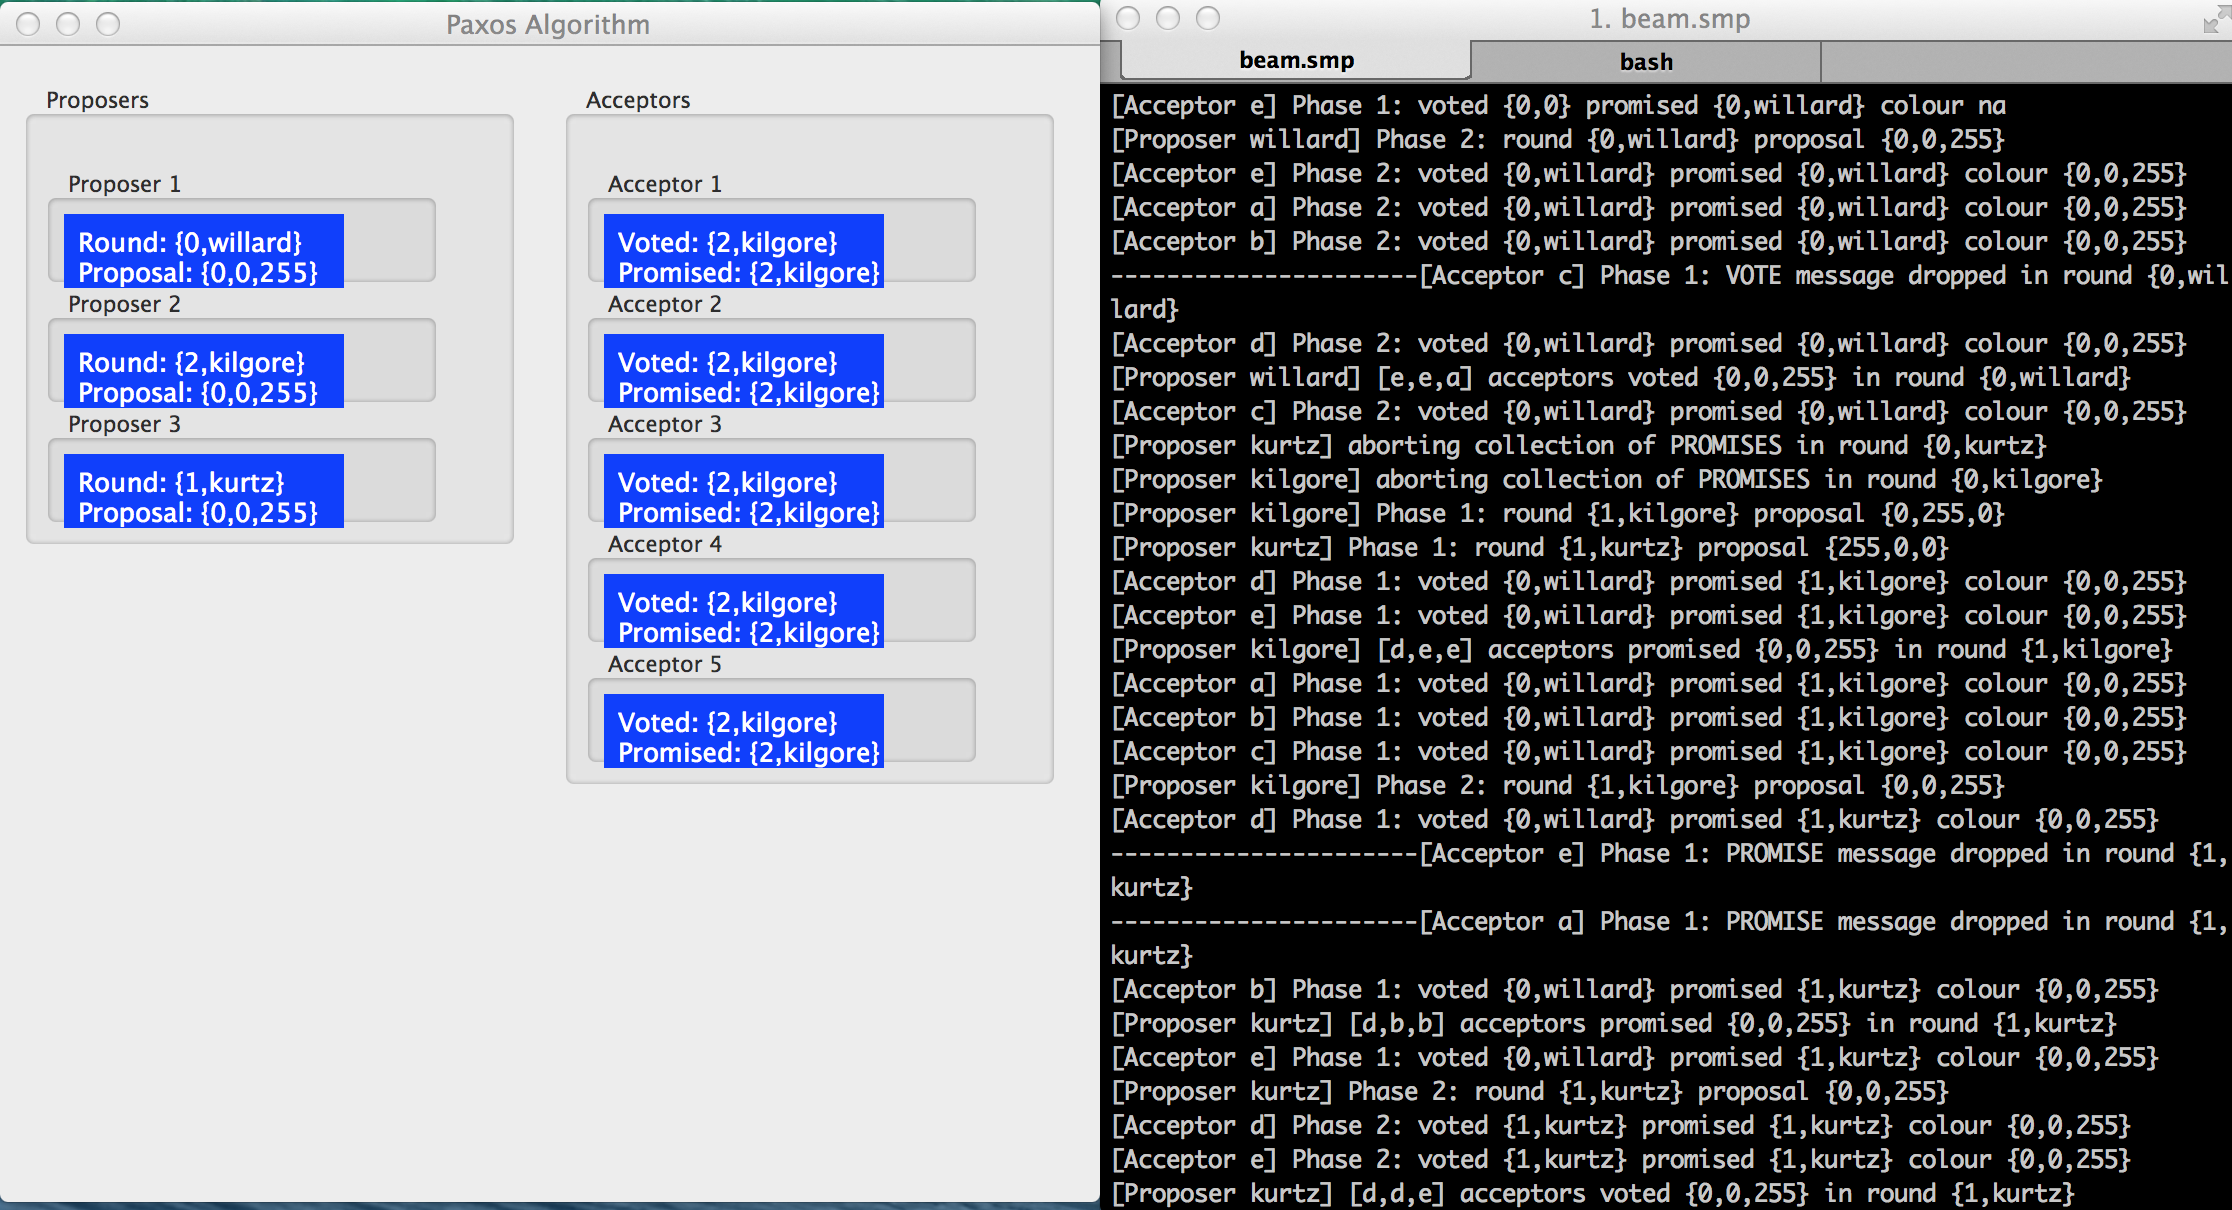
\includegraphics[scale=0.35]{images/exp7.png} \\\\

\textbf{iv)} We increase the number of acceptors to 10 and the number or proposers to 6. The acceptors still get to a consensuns in round 3 on color \textit{purple}.\\
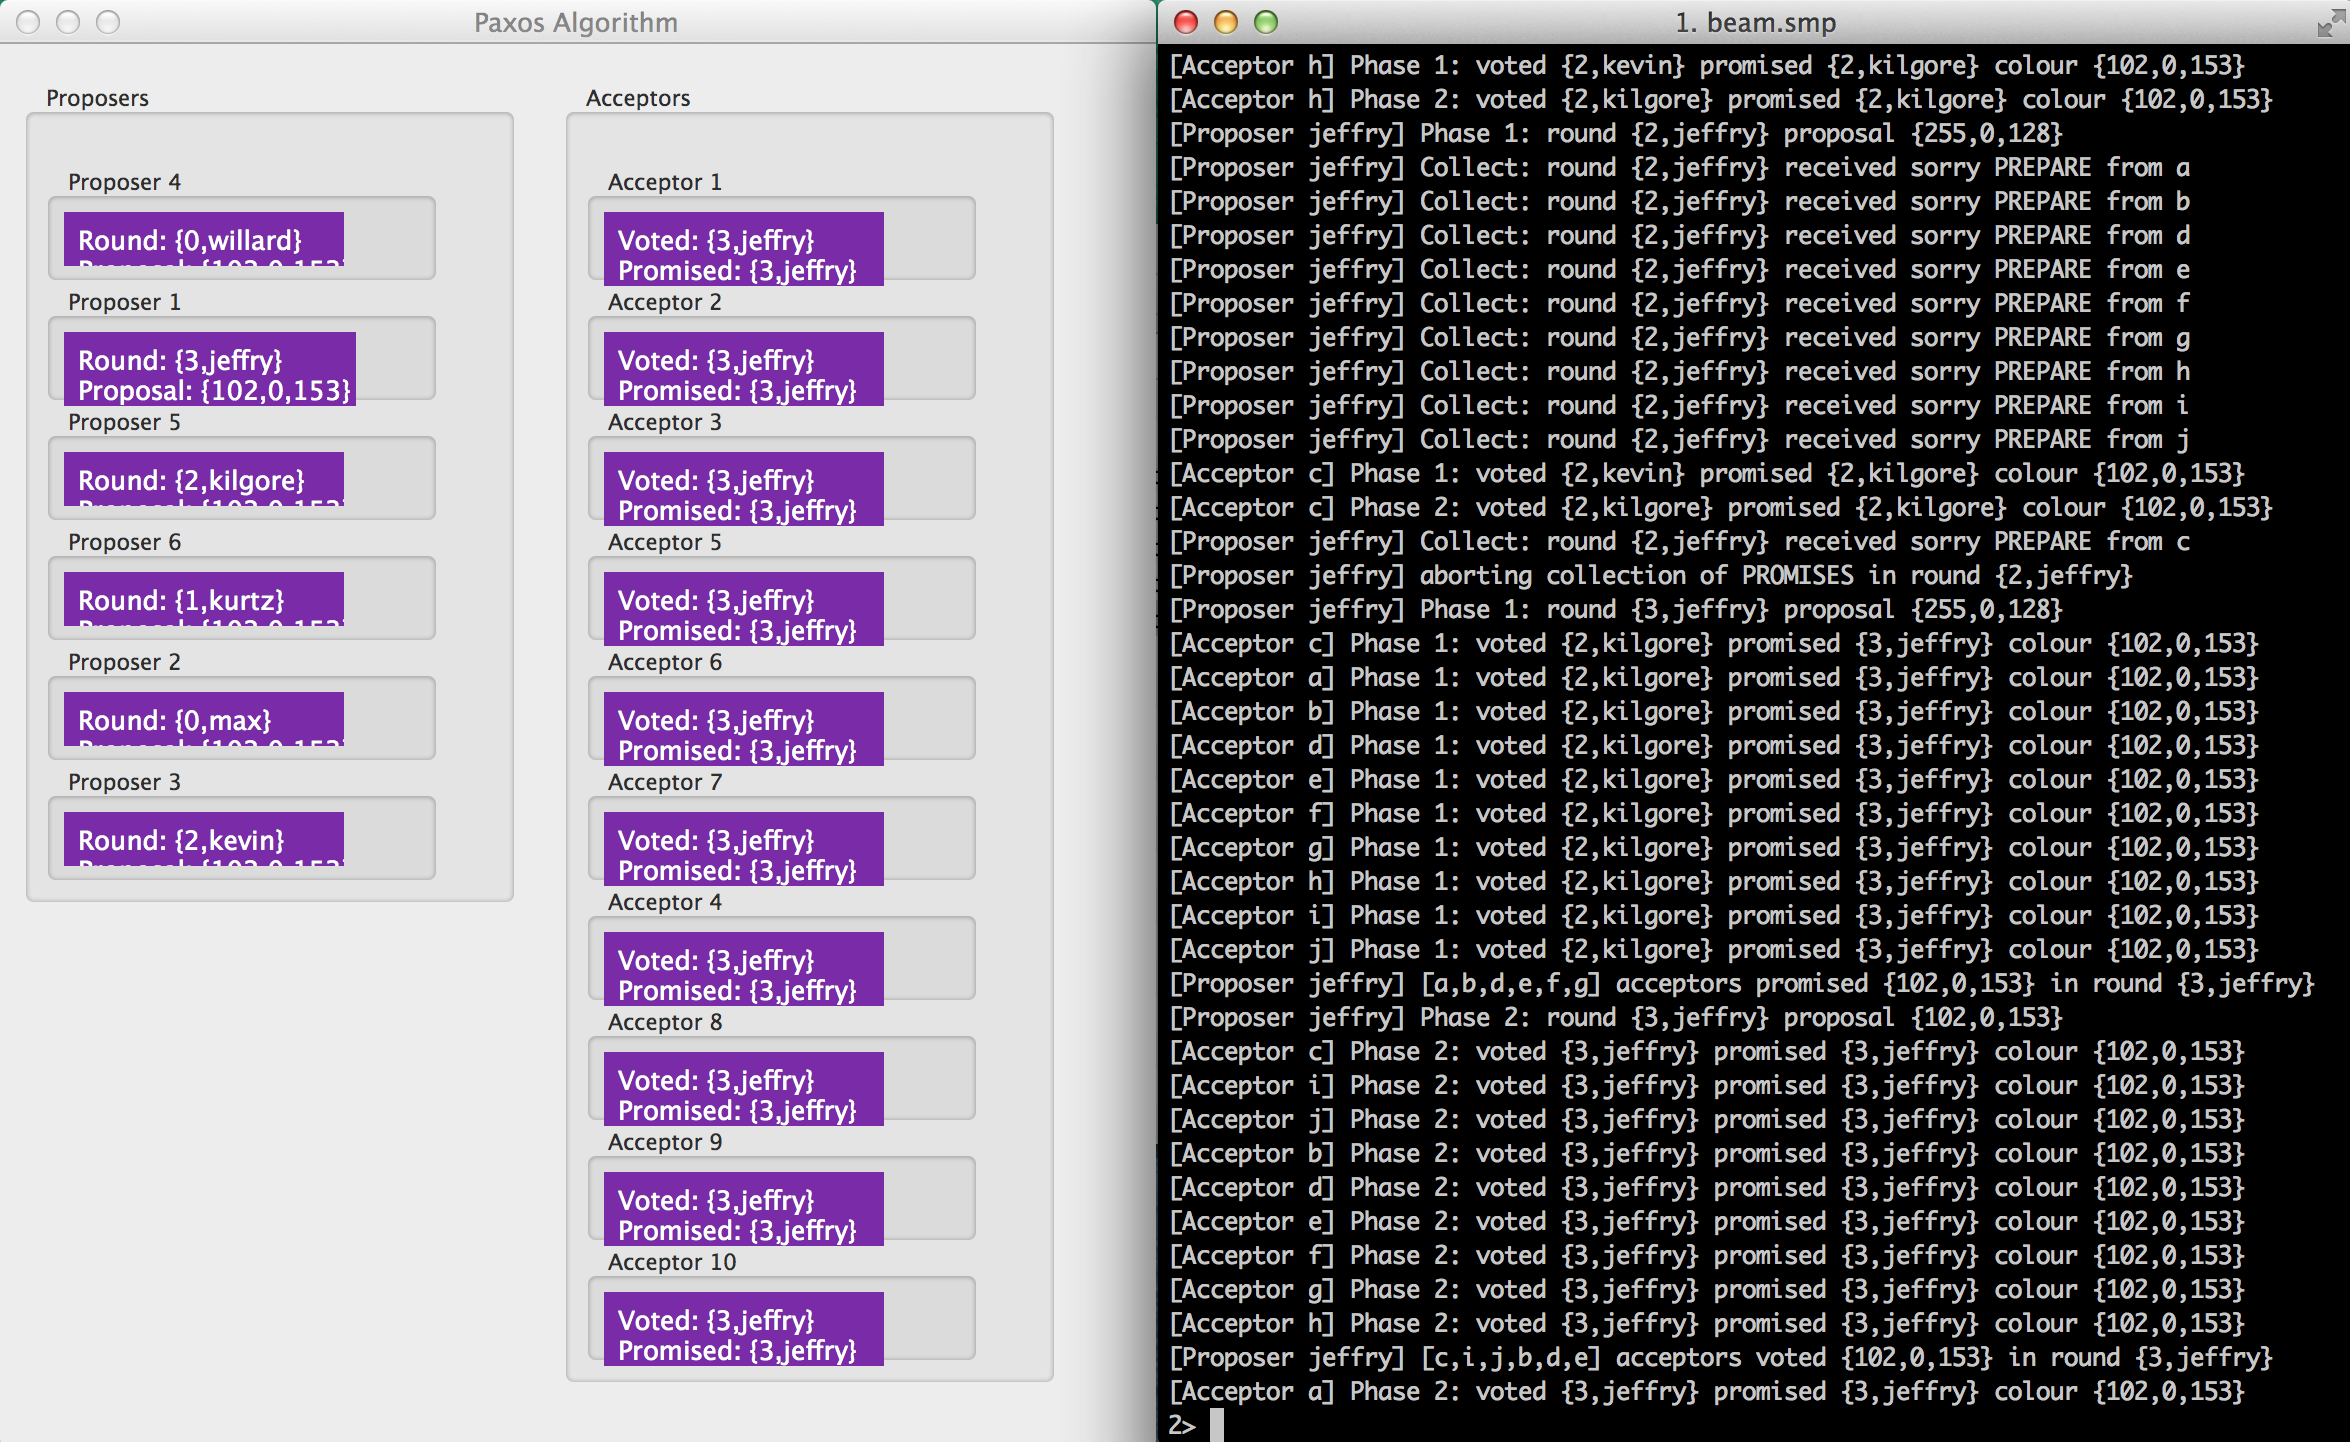
\includegraphics[scale=0.35]{images/exp8.png} \\\\

\textbf{v)} In this experiment we changed the modules to adjust them such that we can run the proposers in one machine and the acceptors in a different one and as they communicate they reach an agreement on the color \textit{blue} in round 2.\\
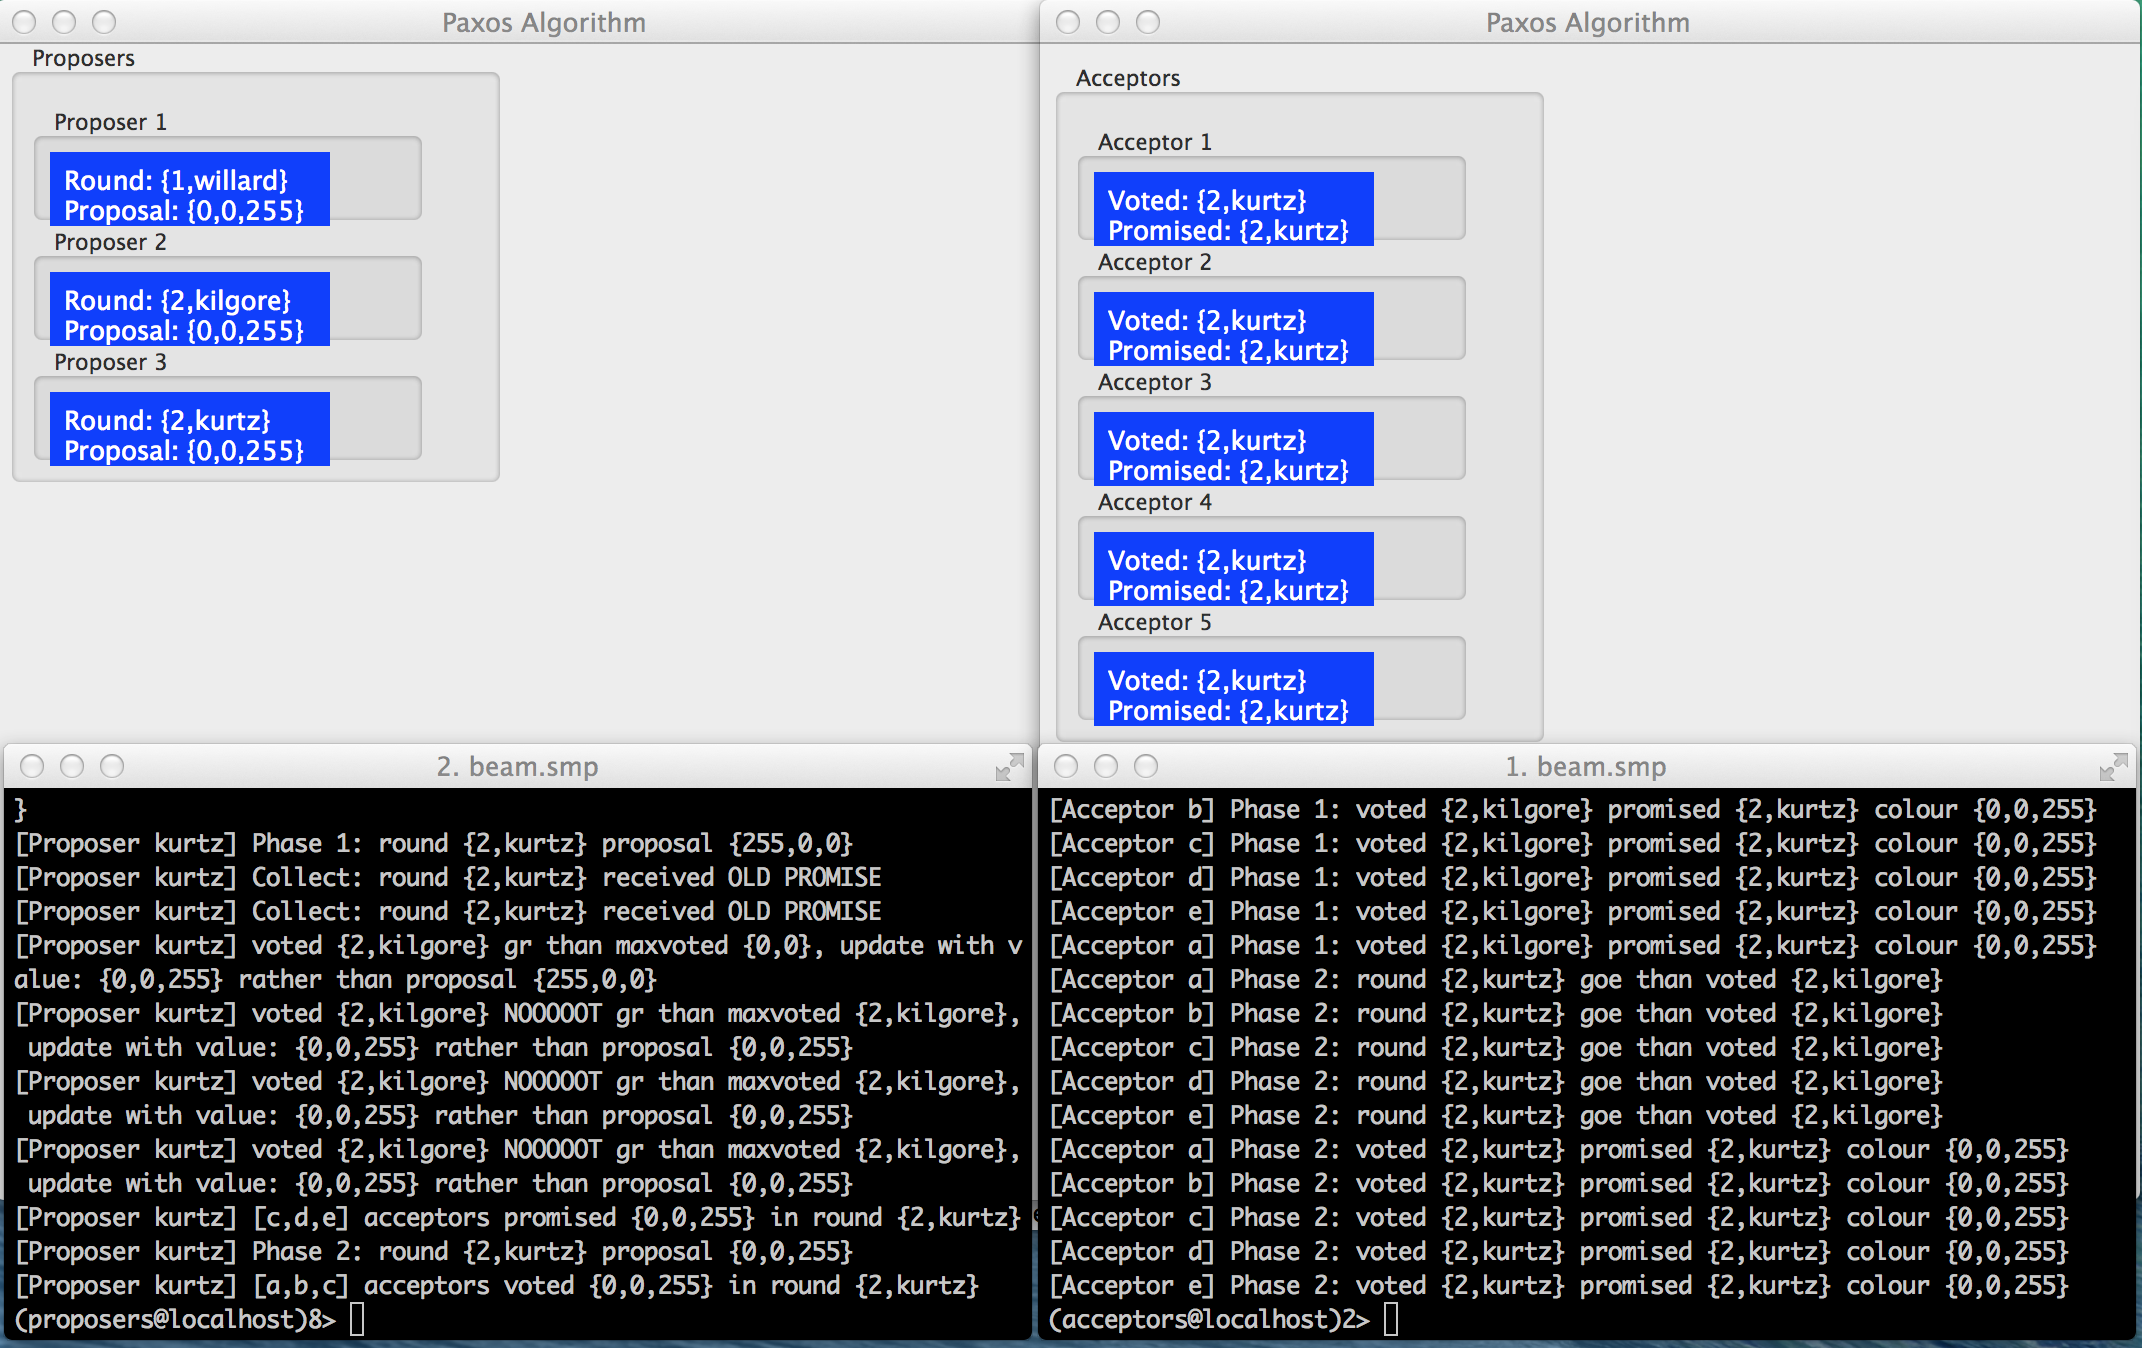
\includegraphics[scale=0.35]{images/exp9.png} \\\\

\textbf{Fault Tollerance}



\section{Open questions}

\textit{Try to answer all the open questions in the documentation. When possible, do experiments to support your answers.}

\section{Personal opinion}

\textit{Provide your personal opinion of the seminar, including whether it should be included in next year's course or not.}

\end{document}
